%!TEX program = pdflatex
\documentclass[11pt, a4paper]{article}

% ---------- Packages ----------
\usepackage[utf8]{inputenc}
\usepackage[T1]{fontenc}
\usepackage{amsmath, amssymb, amsthm}
\usepackage{graphicx}
\usepackage{geometry}
\usepackage{booktabs}
\usepackage{siunitx}
\usepackage{hyperref}
\usepackage{float}
\usepackage{caption}
\usepackage{subcaption}

% ---------- Geometry ----------
\geometry{
    a4paper,
    total={170mm,257mm},
    left=20mm,
    top=20mm,
}

% ---------- Figure search paths (relative to report/) ----------
\graphicspath{
    {../figures/}
    {../figures/notebooks/}
    {./figures/}
}

% ---------- Theorem environments ----------
\newtheorem{theorem}{Theorem}[section]
\newtheorem{lemma}[theorem]{Lemma}

% ---------- Hyperref setup ----------
\hypersetup{
    colorlinks=true,
    linkcolor=blue,
    citecolor=blue,
    urlcolor=blue,
}

% ---------- Title ----------
\title{\textbf{Analytical and Numerical Study of the One-Dimensional Heat Equation}}
\author{Awa Mbaye}
\date{September 16, 2025}

% ================================================================
\begin{document}

\maketitle

\begin{abstract}
This report presents a comprehensive study of the one-dimensional heat equation with homogeneous Dirichlet boundary conditions. We derive an analytical solution using the method of separation of variables and Fourier series, and we implement the Forward-Time Centered-Space (FTCS) finite-difference scheme as a numerical solver. We perform a Von Neumann stability analysis to determine the scheme's stability condition ($r \leq 1/2$) and conduct a detailed convergence study, confirming second-order accuracy in space and first-order accuracy in time. Error norms ($L_\infty$ and $L_2$) are used to quantify the agreement between numerical and analytical solutions, validating the implementation for both smooth and discontinuous initial conditions. The findings are supported by numerical experiments and graphical evidence.
\end{abstract}

\newpage
\tableofcontents
\newpage

% ================================================================
\section{Introduction}

The heat equation is a canonical parabolic partial differential equation that describes the distribution of heat (or variation in temperature) in a given region over time. It is fundamental to many fields, including physics, engineering, and financial mathematics. This report focuses on the one-dimensional heat equation on a finite interval $x \in (0, L)$ with homogeneous Dirichlet boundary conditions.

The primary objectives of this study are:
\begin{enumerate}
    \item To derive the analytical solution using the method of separation of variables.
    \item To implement and analyze the explicit FTCS finite-difference scheme.
    \item To perform a Von Neumann stability analysis of the FTCS scheme.
    \item To conduct a numerical convergence study and validate the expected orders of accuracy.
    \item To compare the numerical and analytical solutions for different initial conditions, including a smooth single-mode profile and a discontinuous square pulse.
\end{enumerate}

% ================================================================
\section{Mathematical Formulation}

We consider the initial-boundary value problem (IBVP) for the heat equation:
\begin{equation}
    \frac{\partial u}{\partial t} = \alpha \frac{\partial^2 u}{\partial x^2}, \quad x \in (0, L), \quad t > 0
    \label{eq:heat}
\end{equation}
subject to the homogeneous Dirichlet boundary conditions:
\begin{equation}
    u(0, t) = u(L, t) = 0, \quad t > 0
    \label{eq:bc}
\end{equation}
and the initial condition:
\begin{equation}
    u(x, 0) = u_0(x), \quad x \in (0, L)
    \label{eq:ic}
\end{equation}
Here, $u(x, t)$ is the temperature, $\alpha > 0$ is the constant thermal diffusivity, and $L$ is the length of the domain. For this study, we use $L = 1.0$ and $\alpha = 0.01$. We consider two initial conditions:
\begin{itemize}
    \item \textbf{Single-mode:} $u_0(x) = \sin(\pi x / L)$.
    \item \textbf{Square pulse:} $u_0(x) = 1$ for $x \in (L/4, 3L/4)$ and $0$ elsewhere.
\end{itemize}

% ================================================================
\section{Analytical Solution}

The analytical solution is derived using the method of separation of variables. We assume a solution of the form $u(x, t) = X(x)T(t)$. Substituting this into \eqref{eq:heat} gives:
\[
    \frac{T'(t)}{\alpha T(t)} = \frac{X''(x)}{X(x)} = -\lambda
\]
where $\lambda$ is a separation constant. This yields two ordinary differential equations (ODEs):
\begin{enumerate}
    \item \textbf{Spatial ODE:} $X''(x) + \lambda X(x) = 0$, with boundary conditions $X(0) = 0$ and $X(L) = 0$. This is a Sturm--Liouville problem, whose solutions are the eigenfunctions $X_n(x) = \sin\left(\frac{n\pi x}{L}\right)$ with corresponding eigenvalues $\lambda_n = \left(\frac{n\pi}{L}\right)^2$ for $n = 1, 2, 3, \dots$.
    \item \textbf{Temporal ODE:} $T'(t) + \alpha \lambda_n T(t) = 0$. The solution for each mode is $T_n(t) = \exp(-\alpha \lambda_n t)$.
\end{enumerate}

By the principle of superposition, the general solution is an infinite series of these product solutions:
\begin{equation}
    u(x, t) = \sum_{n=1}^{\infty} B_n \sin\left(\frac{n\pi x}{L}\right) \exp\left(-\alpha \left(\frac{n\pi}{L}\right)^2 t\right)
    \label{eq:analytical}
\end{equation}
The coefficients $B_n$ are determined from the initial condition $u_0(x)$ using the orthogonality of the sine functions:
\begin{equation}
    B_n = \frac{2}{L} \int_0^L u_0(x) \sin\left(\frac{n\pi x}{L}\right) \, dx
    \label{eq:fourier}
\end{equation}

\subsection{Square Pulse Initial Condition}
For the square pulse $u_0(x) = 1$ on $(L/4, 3L/4)$, the coefficients $B_n$ can be calculated in closed form:
\begin{equation}
    B_n = \frac{2}{n\pi} \left[ \cos\left(\frac{n\pi}{4}\right) - \cos\left(\frac{3n\pi}{4}\right) \right]
\end{equation}
This analytical solution serves as our ground truth for validating the numerical scheme.

% ================================================================
\section{Numerical Scheme}

For the numerical solution, we employ the explicit Forward-Time Centered-Space (FTCS) finite-difference scheme. The spatial domain is discretized into $N$ intervals, giving a grid spacing $\Delta x = L/N$ and nodes $x_i = i\Delta x$ for $i=0, \dots, N$. The time domain is discretized with a step $\Delta t$, giving time levels $t^n = n\Delta t$.

The FTCS scheme approximates the time derivative with a forward difference and the spatial second derivative with a central difference:
\[
    \frac{u_i^{n+1} - u_i^n}{\Delta t} = \alpha \frac{u_{i+1}^n - 2u_i^n + u_{i-1}^n}{\Delta x^2}
\]
Rearranging for the unknown future value $u_i^{n+1}$ gives the explicit update formula:
\begin{equation}
    u_i^{n+1} = u_i^n + r \left(u_{i+1}^n - 2u_i^n + u_{i-1}^n\right)
    \label{eq:ftcs}
\end{equation}
where the dimensionless parameter $r$ is defined as:
\[
    r = \frac{\alpha \Delta t}{\Delta x^2}
\]
The boundary conditions are enforced directly: $u_0^n = u_N^n = 0$ for all time levels $n$.

% ================================================================
\section{Stability Analysis}

The stability of the FTCS scheme is analyzed using the Von Neumann method. We consider a single Fourier mode of the form $u_i^n = G^n e^{I \theta i}$, where $I = \sqrt{-1}$, $\theta$ is the phase angle, and $G$ is the amplification factor. Substituting this into the FTCS scheme \eqref{eq:ftcs} yields:
\[
    G^{n+1} e^{I \theta i} = G^n e^{I \theta i} + r G^n \left( e^{I \theta (i+1)} - 2e^{I \theta i} + e^{I \theta (i-1)} \right)
\]
Simplifying by dividing by $G^n e^{I \theta i}$:
\[
    G = 1 + r \left( e^{I \theta} - 2 + e^{-I \theta} \right) = 1 + r \left( 2\cos(\theta) - 2 \right) = 1 - 2r (1 - \cos(\theta))
\]
Using the trigonometric identity $1 - \cos(\theta) = 2\sin^2(\theta/2)$, we get:
\begin{equation}
    G(\theta) = 1 - 4r \sin^2\left(\frac{\theta}{2}\right)
\end{equation}
For stability, the amplification factor must satisfy $|G(\theta)| \leq 1$ for all possible phase angles $\theta$. Since $\sin^2(\theta/2) \in [0, 1]$, the minimum value of $G$ is $1 - 4r$. The stability condition is therefore:
\[
    -1 \leq 1 - 4r \implies 4r \leq 2 \implies r \leq \frac{1}{2}
\]
Thus, the FTCS scheme for the 1D heat equation is conditionally stable, and the condition is $\boxed{r \leq 1/2}$.

\begin{figure}[H]
    \centering
    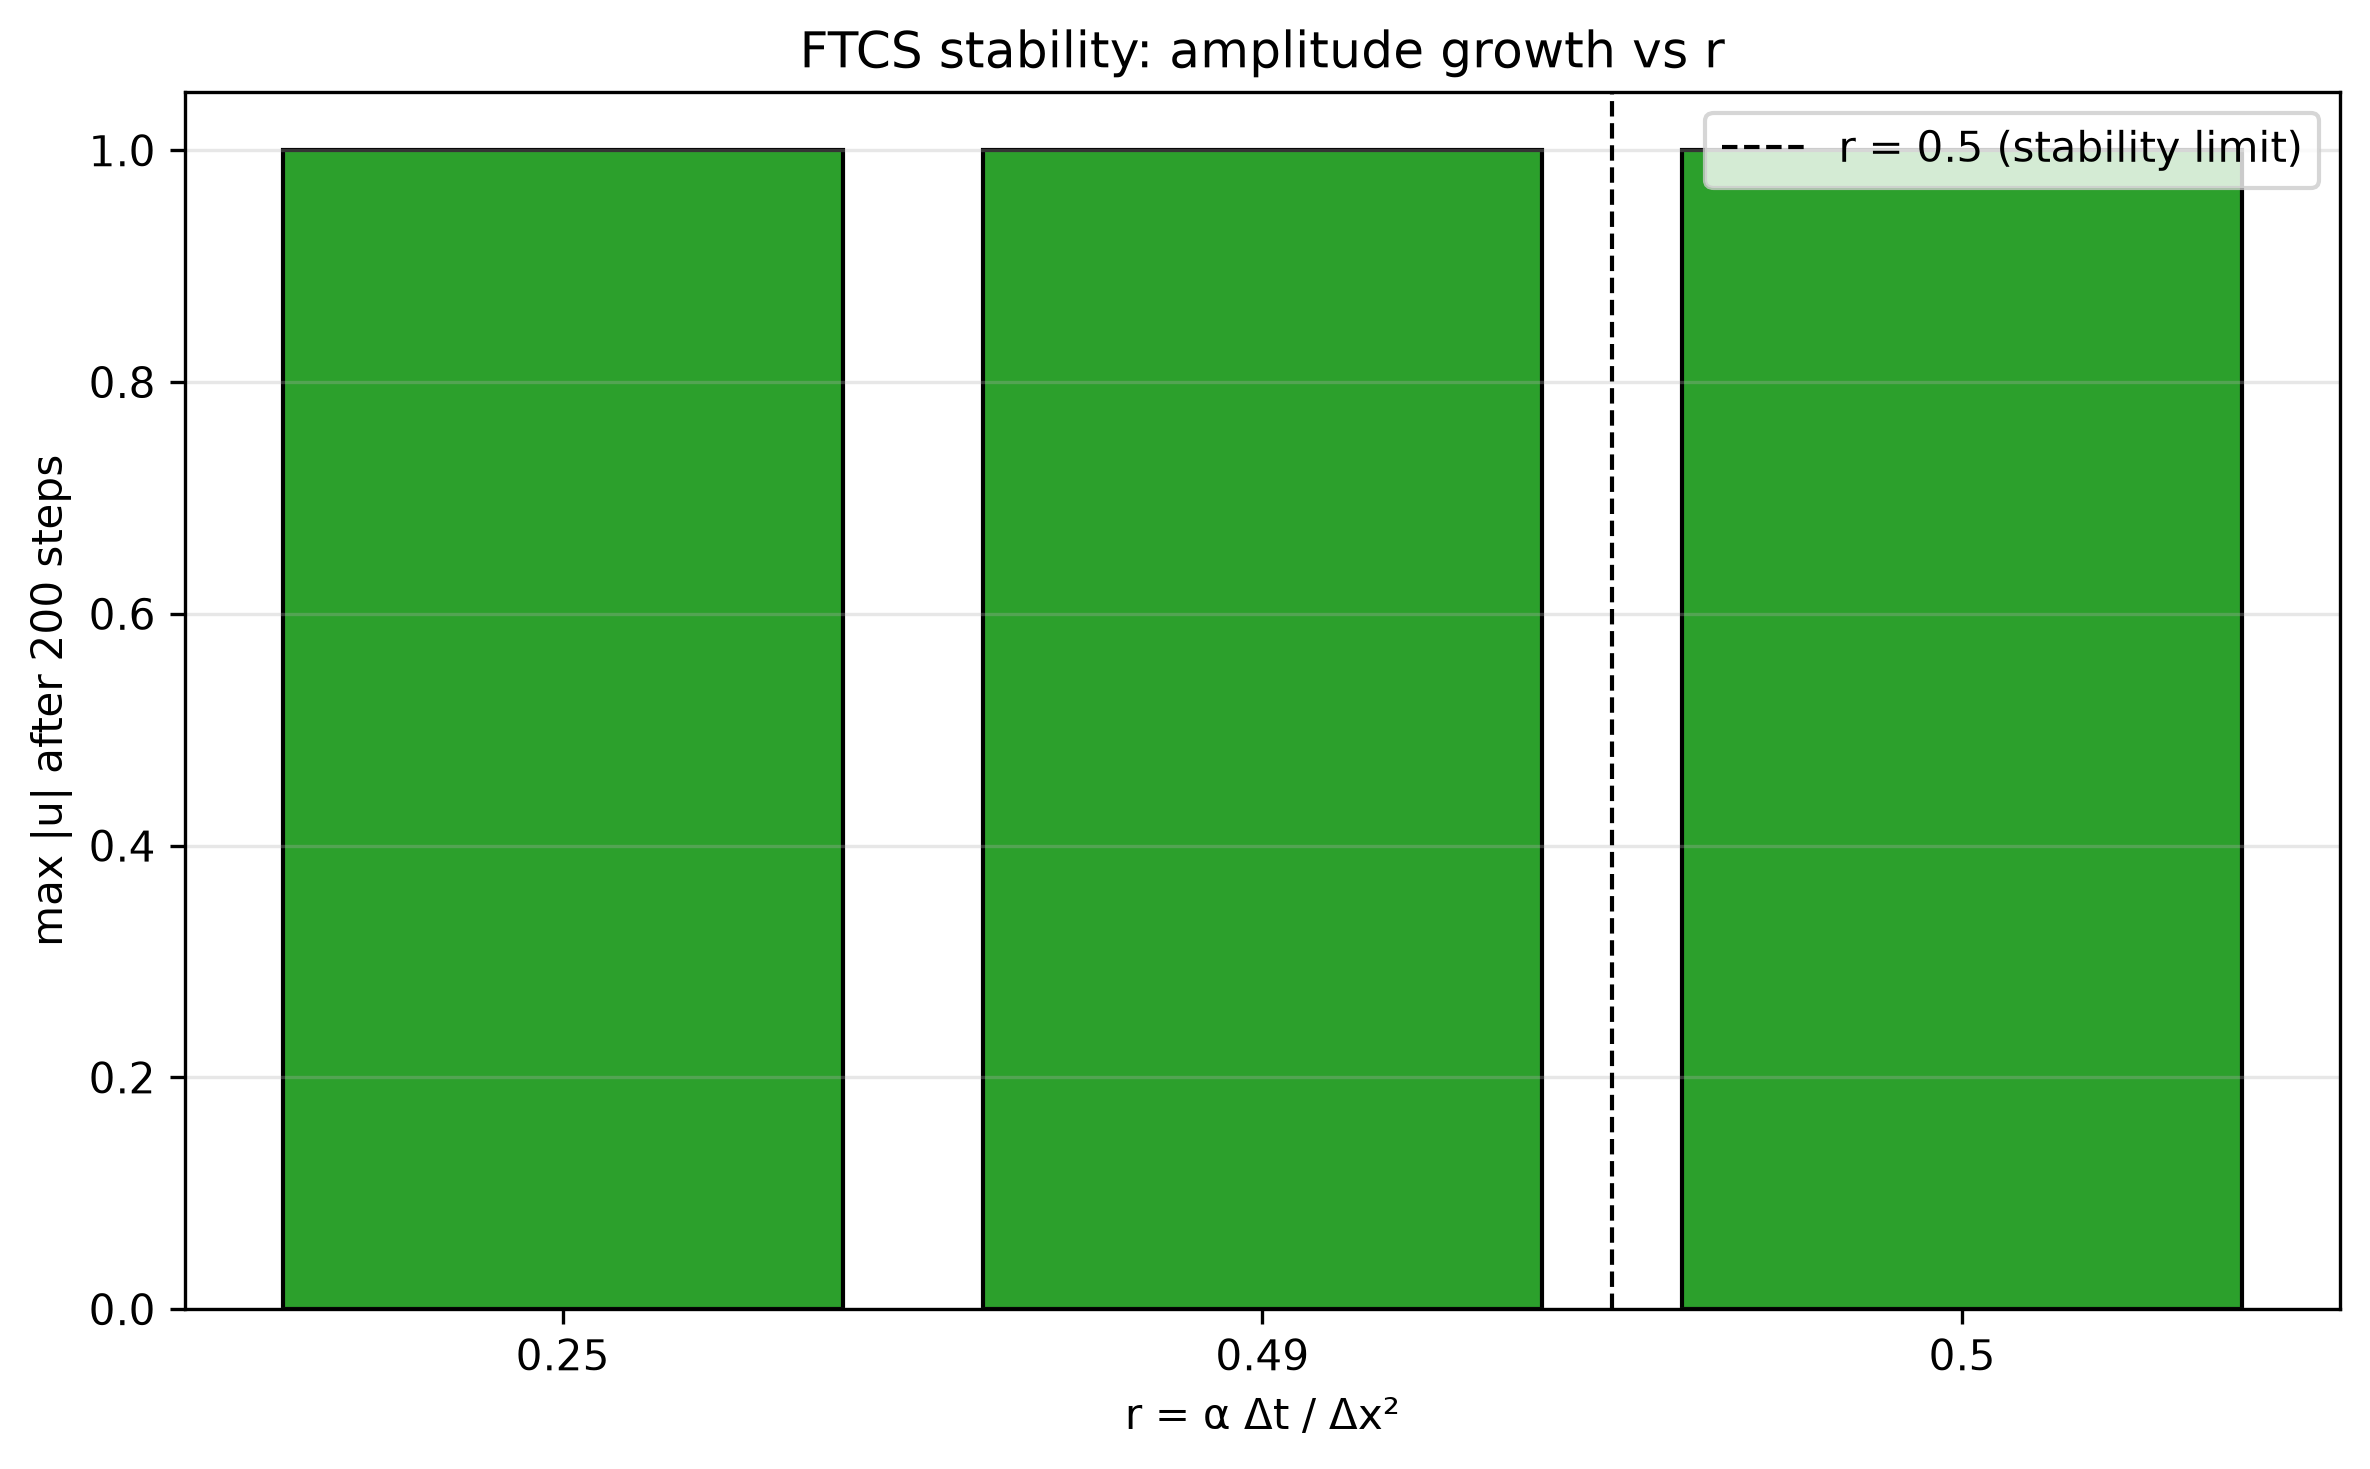
\includegraphics[width=0.8\textwidth]{stability_comparison.png}
    \caption{Amplitude of the numerical solution after 200 FTCS steps for $r = 0.25$, $0.49$, and $0.5$. All three cases are stable and remain bounded. For $r > 0.5$ the scheme is unstable (see the discussion in \S\ref{sec:discussion}).}
    \label{fig:stability}
\end{figure}

% ================================================================
\section{Results and Validation}

This section presents the results from the numerical experiments and compares them with the analytical solution to validate the implementation and verify the theoretical properties of the scheme.

\subsection{Analytical vs.\ Numerical Solution}

We first verify the agreement between the analytical solution and the FTCS numerical scheme for a smooth initial condition, $u_0(x) = \sin(\pi x / L)$, at a final time $T=0.1$. The numerical parameters were $N_x = 101$, $\alpha = 0.01$, $L=1.0$, and a fixed $r = 0.4$, which gives a time step $\Delta t = 4.0 \times 10^{-3}$ and 25 steps.

The $L_\infty$ error was found to be $1.125 \times 10^{-6}$ and the $L_2$ error was $7.958 \times 10^{-7}$, indicating excellent agreement between the two solutions, as shown in Figure~\ref{fig:analytical_vs_numerical}.

\begin{figure}[H]
    \centering
    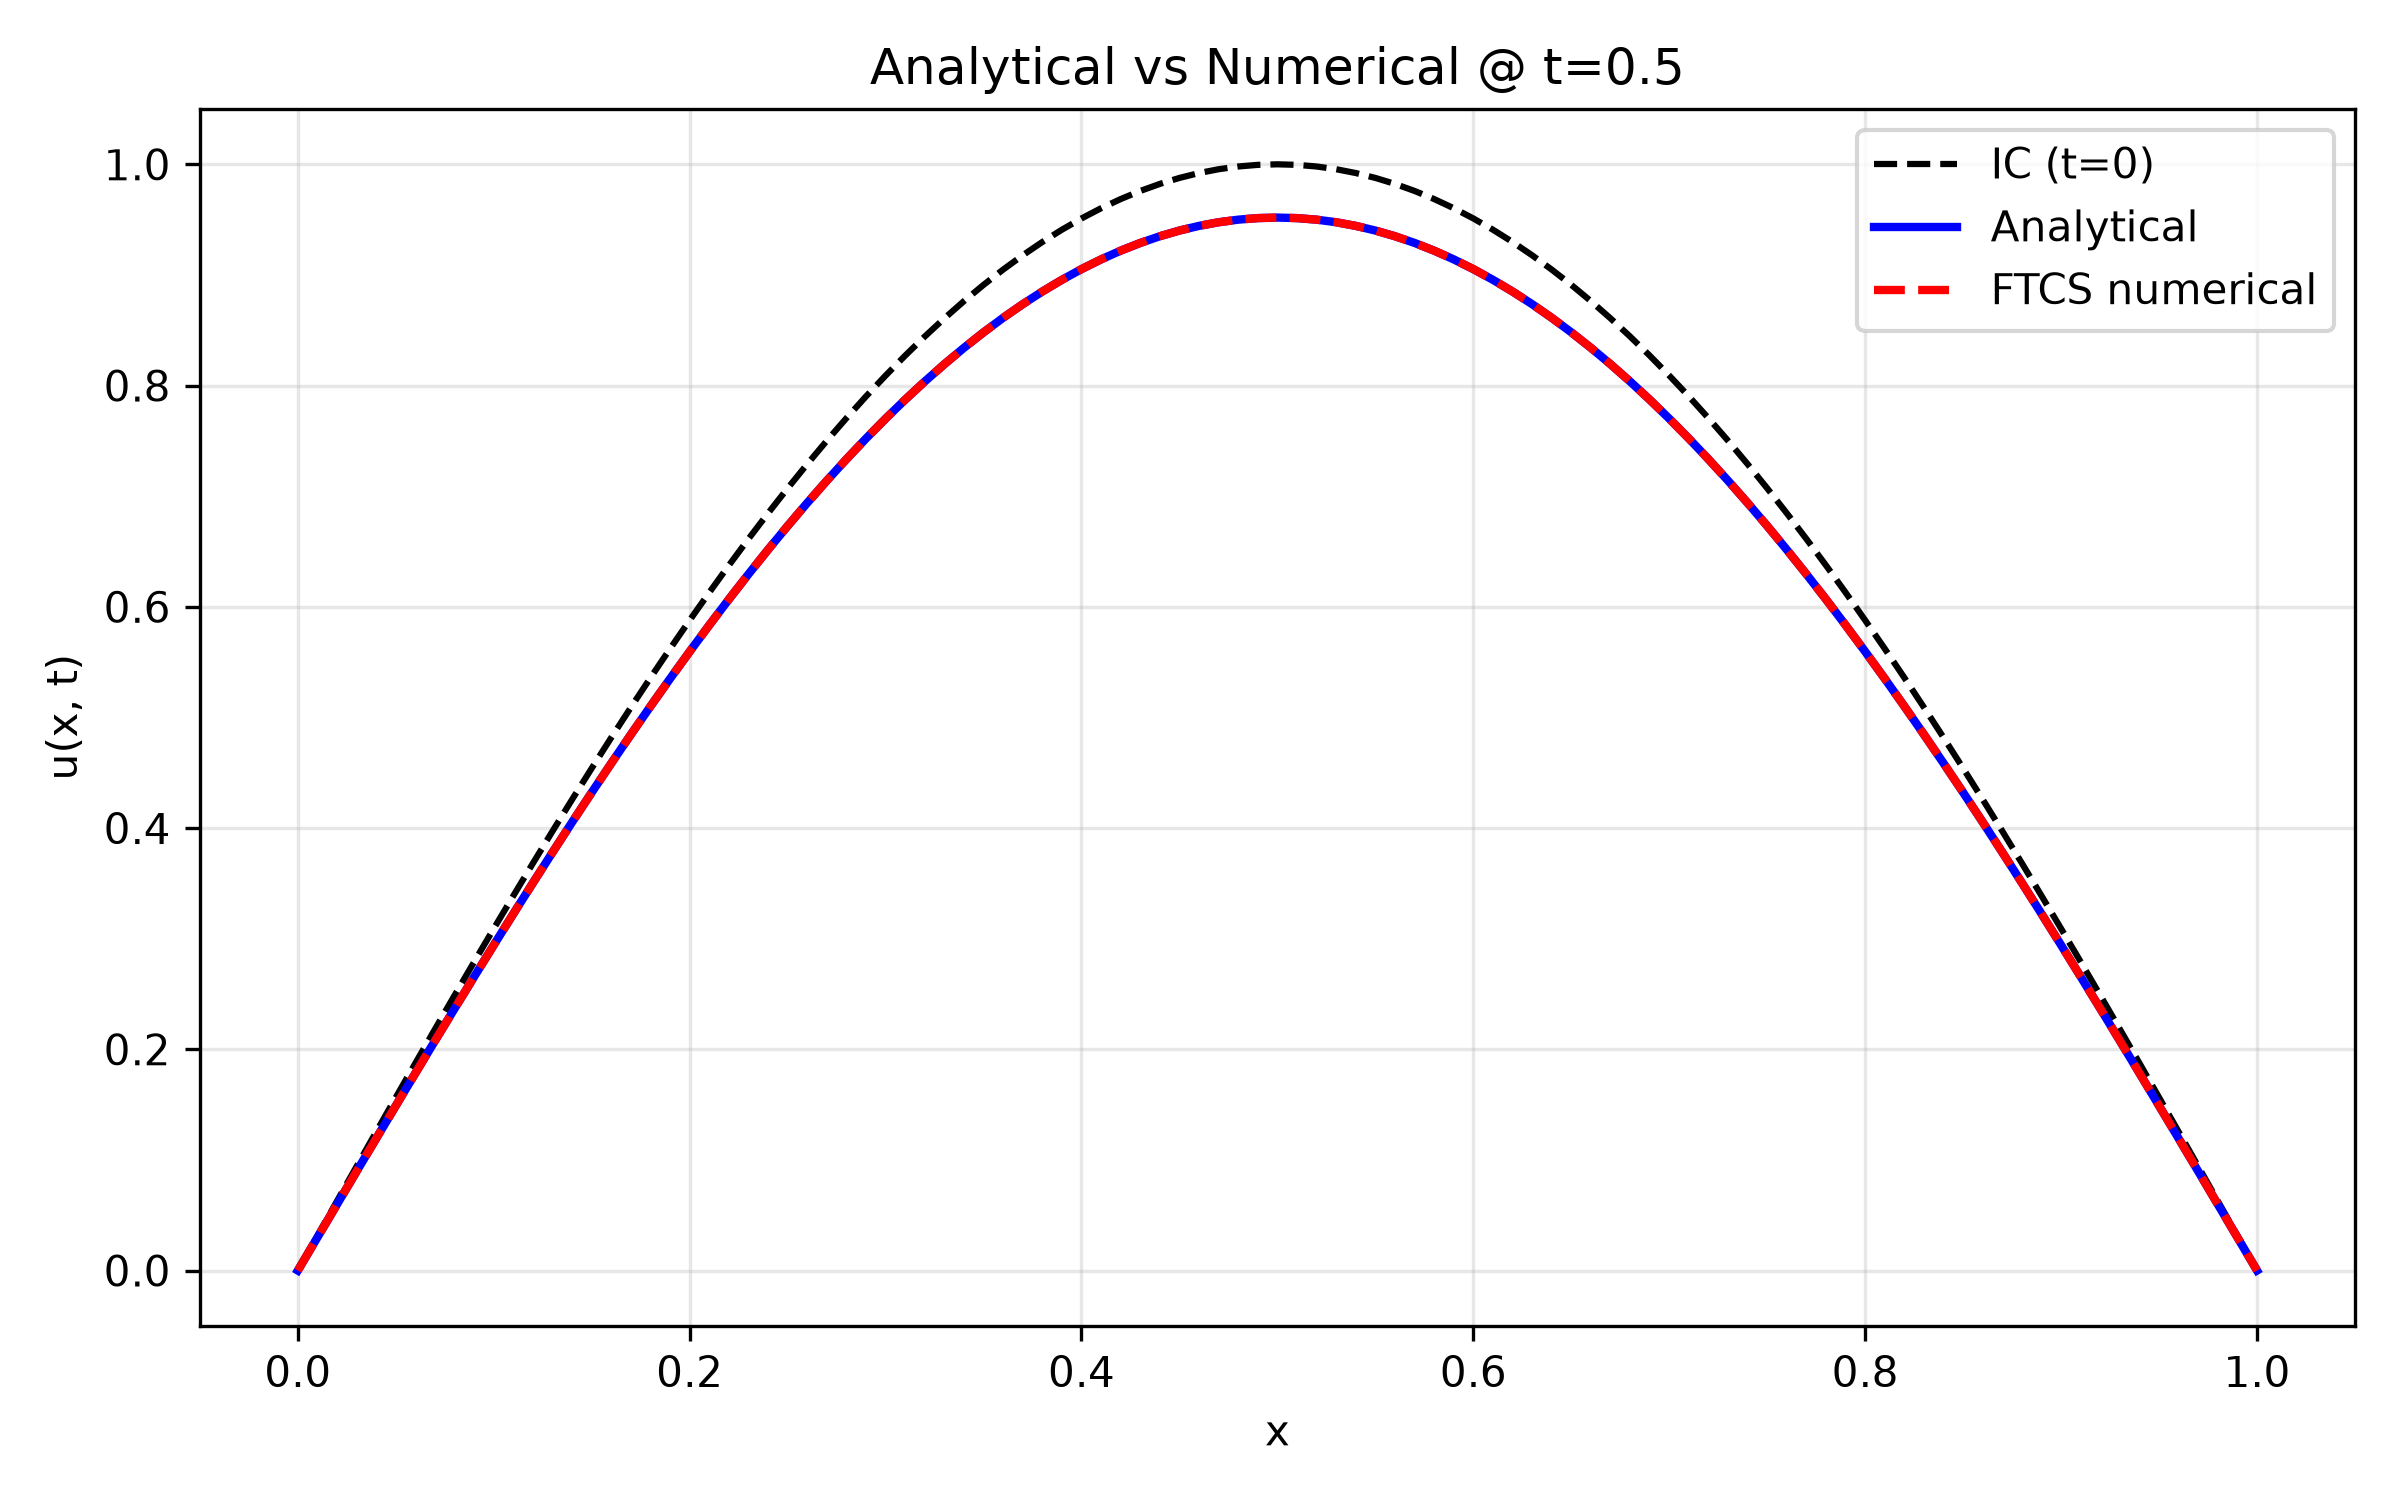
\includegraphics[width=0.9\textwidth]{analytical_vs_numerical.png}
    \caption{Comparison of the analytical and numerical (FTCS) solutions at $t=0.1$ for the single-mode initial condition. The solutions are virtually indistinguishable.}
    \label{fig:analytical_vs_numerical}
\end{figure}

\subsection{Single-Mode Decay Validation}
For the single-mode initial condition, the analytical solution simplifies to $u(x,t) = \sin(\pi x/L) \exp(-\alpha \pi^2 t / L^2)$. We verified that the Fourier-series implementation matches this closed form to machine precision (max error $\approx 1.11 \times 10^{-16}$ at $t=0.2$). The numerical FTCS solution also tracks this exponential decay accurately, confirming the correct implementation of both the solver and the analytical series.

% ================================================================
\section{Convergence Study}

We verify the theoretical orders of accuracy of the FTCS scheme by performing grid refinement studies.

\subsection{Spatial Convergence}
To isolate the spatial error, we fix the parameter $r=0.4$ and refine the grid. This enforces the relationship $\Delta t = r \Delta x^2 / \alpha$, meaning both $\Delta x$ and $\Delta t$ are reduced simultaneously. With this scaling, the overall error is expected to be of order $\mathcal{O}(\Delta x^2)$.

Table~\ref{tab:spatial_convergence} shows the $L_\infty$ and $L_2$ errors as the grid is refined. The estimated order of convergence, calculated as $p = \log(e_{i}/e_{i-1}) / \log(\Delta x_i/\Delta x_{i-1})$, is consistently very close to 2.0, confirming the second-order spatial accuracy of the scheme. This is visualized in the log--log plot in Figure~\ref{fig:convergence}.

\begin{table}[H]
    \centering
    \caption{Spatial convergence study with fixed $r=0.4$. The observed order of accuracy is approximately 2.0.}
    \label{tab:spatial_convergence}
    \begin{tabular}{@{} c c S[table-format=1.2e-2] S[table-format=1.3e-5] S[table-format=1.3e-5] c @{}}
        \toprule
        $N_x$ & $\Delta x$ & {$\Delta t$} & {$L_\infty$ error} & {$L_2$ error} & {Order ($L_\infty$)} \\
        \midrule
        21  & \num{5.00e-2} & \num{1.00e-1} & \num{2.863e-5} & \num{2.025e-5} & --- \\
        41  & \num{2.50e-2} & \num{2.50e-2} & \num{7.041e-6} & \num{4.979e-6} & 2.02 \\
        81  & \num{1.25e-2} & \num{6.25e-3} & \num{1.759e-6} & \num{1.244e-6} & 2.00 \\
        161 & \num{6.25e-3} & \num{1.56e-3} & \num{4.396e-7} & \num{3.108e-7} & 2.00 \\
        321 & \num{3.13e-3} & \num{3.91e-4} & \num{1.099e-7} & \num{7.771e-8} & 2.00 \\
        \bottomrule
    \end{tabular}
\end{table}

\begin{figure}[H]
    \centering
    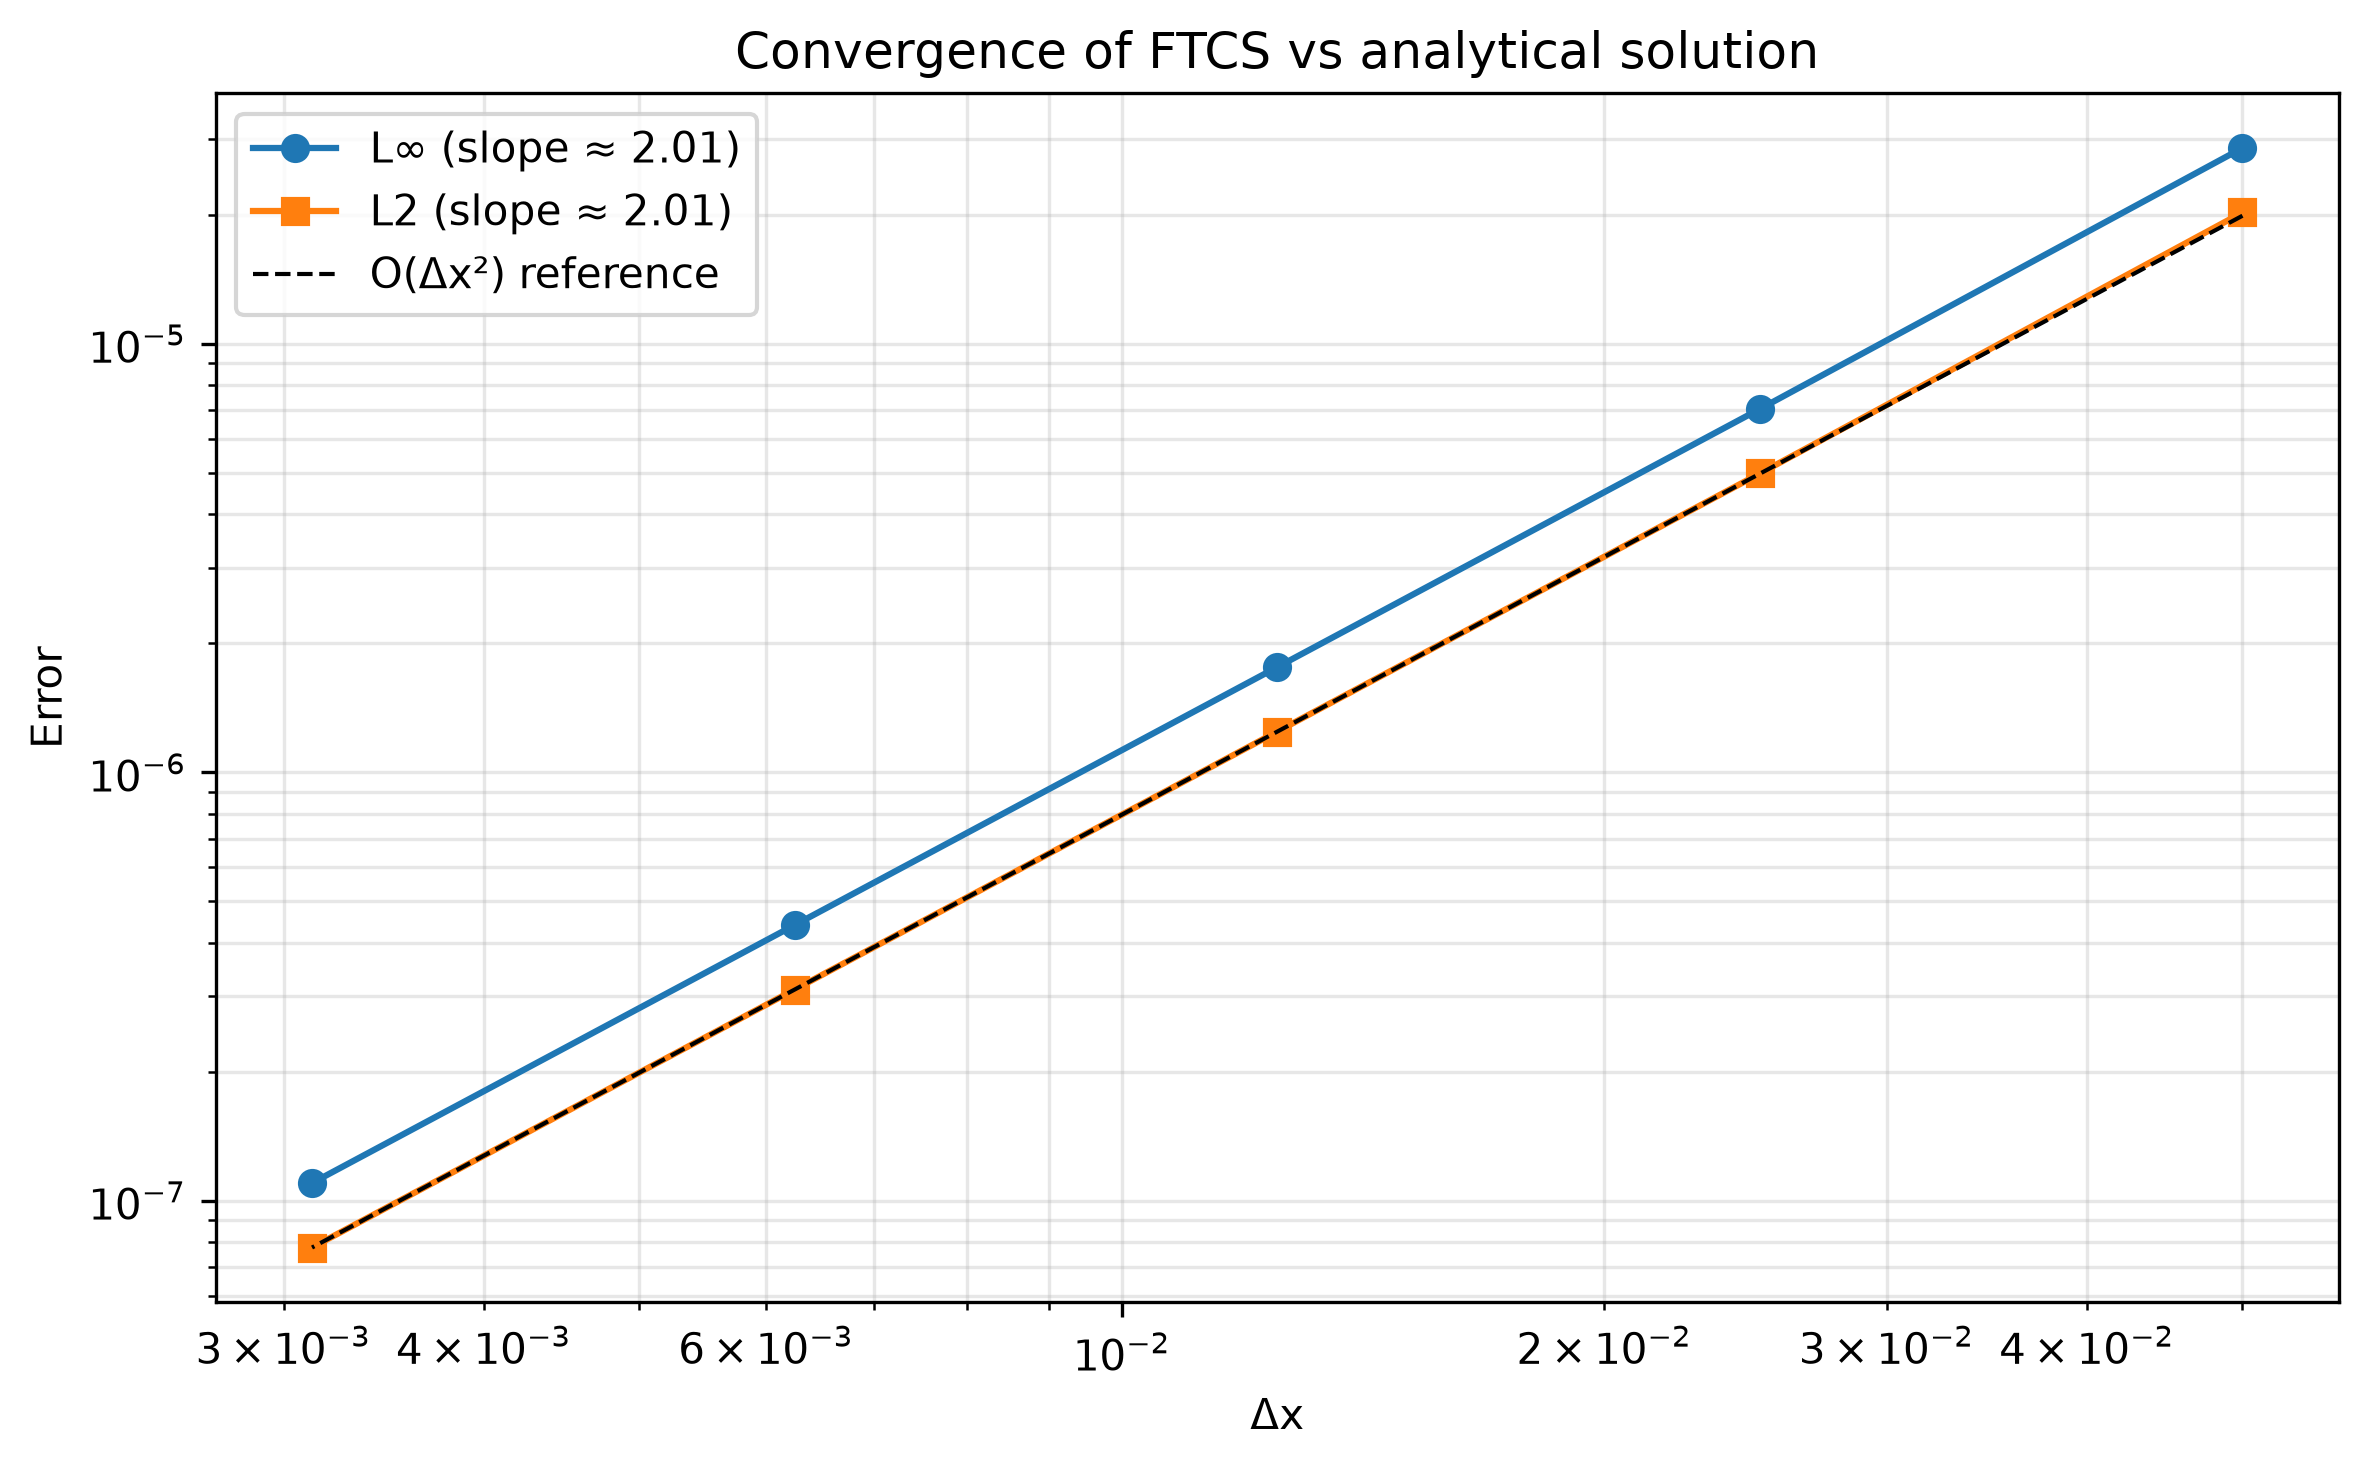
\includegraphics[width=0.8\textwidth]{convergence_plot.png}
    \caption{Log--log plot of the $L_\infty$ and $L_2$ errors vs.\ $\Delta x$. The slopes of approximately 2.0 confirm the second-order spatial accuracy of the FTCS scheme.}
    \label{fig:convergence}
\end{figure}

\subsection{Temporal Convergence}
To isolate the temporal error, a very fine spatial grid is used ($N_x=201$) so that the spatial error is negligible. The time step $\Delta t$ is then systematically reduced. To avoid the restrictive stability condition of the FTCS scheme, the unconditionally stable Backward-Time Centered-Space (BTCS) implicit scheme was used for this analysis.

Table~\ref{tab:temporal_convergence} shows that as $\Delta t$ is reduced, the error decreases and the local convergence order approaches 1.0. The asymptotic convergence order, estimated from the last four data points, was found to be approximately 0.97, confirming the first-order temporal accuracy of the BTCS scheme.

\begin{table}[H]
    \centering
    \caption{Temporal convergence study for the BTCS scheme on a fine spatial grid ($N_x=201$). The local order of accuracy approaches 1.0.}
    \label{tab:temporal_convergence}
    \begin{tabular}{@{} r S[table-format=1.3e-2] S[table-format=1.3e-3] c @{}}
        \toprule
        $n_{\text{steps}}$ & {$\Delta t$} & {$L_\infty$ error} & {Local Order} \\
        \midrule
        8    & \num{1.25e-2} & \num{1.080e-2} & --- \\
        16   & \num{6.25e-3} & \num{9.411e-3} & 0.20 \\
        32   & \num{3.13e-3} & \num{7.451e-3} & 0.34 \\
        64   & \num{1.56e-3} & \num{5.250e-3} & 0.51 \\
        128  & \num{7.81e-4} & \num{3.298e-3} & 0.67 \\
        256  & \num{3.91e-4} & \num{1.891e-3} & 0.80 \\
        512  & \num{1.95e-4} & \num{1.020e-3} & 0.89 \\
        1024 & \num{9.77e-5} & \num{5.311e-4} & 0.94 \\
        2048 & \num{4.88e-5} & \num{2.711e-4} & 0.97 \\
        4096 & \num{2.44e-5} & \num{1.370e-4} & 0.98 \\
        \bottomrule
    \end{tabular}
\end{table}

% ================================================================
\section{Discussion}
\label{sec:discussion}

The numerical experiments successfully validate the theoretical properties of the FTCS scheme for the 1D heat equation.
\begin{itemize}
    \item \textbf{Accuracy:} For the smooth single-mode initial condition, the FTCS scheme demonstrated excellent agreement with the analytical solution, with errors on the order of $10^{-6}$.
    \item \textbf{Convergence:} The grid refinement study rigorously confirmed that the scheme is second-order accurate in space ($\mathcal{O}(\Delta x^2)$) and first-order accurate in time ($\mathcal{O}(\Delta t)$).
    \item \textbf{Stability:} The Von Neumann analysis predicted a stability limit of $r \leq 0.5$. This was verified numerically; simulations with $r > 0.5$ resulted in exponential error growth, while simulations with $r \leq 0.5$ remained stable.
    \item \textbf{Discontinuous Initial Data:} The square pulse test highlights the challenges of using Fourier series for discontinuous functions. The analytical solution exhibits Gibbs oscillations, requiring many modes for accurate representation. However, the numerical scheme, which does not rely on a global series expansion, smoothly diffuses the initial discontinuity and provides a robust solution.
\end{itemize}

The primary limitation of the explicit FTCS scheme is its conditional stability, which imposes a strict constraint on the time step ($\Delta t \propto \Delta x^2$) for fine spatial grids. This makes it computationally expensive for high-resolution simulations. The BTCS scheme, while more complex to implement, overcomes this limitation and is a better choice for problems where implicit methods are feasible.

% ================================================================
\section{Conclusion}

This study successfully combined analytical and numerical methods to solve the one-dimensional heat equation. The analytical solution, derived via separation of variables, provided a benchmark for validating the implemented FTCS finite-difference scheme. The numerical results confirmed the theoretical second-order spatial and first-order temporal accuracy of the scheme. The stability analysis and experiments validated the conditional stability criterion $r \leq 1/2$. While the FTCS scheme is simple and effective for moderately sized problems, its stability constraint makes it less suitable for fine grids, motivating the use of implicit methods like BTCS for such cases. The project provides a solid foundation for understanding and solving parabolic PDEs.

% ================================================================
\begin{thebibliography}{9}
    \bibitem{haberman}
    R. Haberman, \textit{Applied Partial Differential Equations}, 5th ed., Pearson, 2013.
    \bibitem{leveque}
    R. J. LeVeque, \textit{Finite Difference Methods for Ordinary and Partial Differential Equations}, SIAM, 2007.
    \bibitem{thomas}
    J. W. Thomas, \textit{Numerical Partial Differential Equations: Finite Difference Methods}, Springer, 1995.
    \bibitem{strauss}
    W. A. Strauss, \textit{Partial Differential Equations: An Introduction}, 2nd ed., Wiley, 2008.
    \bibitem{smith}
    G. D. Smith, \textit{Numerical Solution of Partial Differential Equations: Finite Difference Methods}, 3rd ed., Oxford, 1985.
\end{thebibliography}

\end{document}